\documentclass[12pt]{article}

\usepackage[utf8]{inputenc}
\usepackage[a4paper, margin=1in]{geometry}
\usepackage{booktabs}
\usepackage{physics}
\usepackage{amsmath}
\usepackage{amsfonts}
\usepackage{graphicx}
\usepackage{siunitx}
\usepackage{multirow}

\graphicspath{{./figures}}

\title{Physical Climatology (AES 630) Project 3}
\author{Mitchell Dodson}
\date{November 4, 2023}

\newcommand*{\problem}[2]{
    \begin{table}[ht]
    \centering
        \begin{tabular}{ | p{.1\linewidth} p{.9\linewidth} | }
            \hline
            \vspace{.3em}\textbf{\large#1:} & \vspace{.3em}\footnotesize{#2}\hspace{.2em}\vspace{.5em} \\ \hline
        \end{tabular}
    \end{table}
}


\newcommand\T{\rule{0pt}{2.6ex}}       % Top strut
\newcommand\B{\rule[-1.2ex]{0pt}{0pt}} % Bottom strut

\begin{document}

\vspace{-2em}

\maketitle

\vspace{-2em}

\section{Solar Reflectivity}

\begin{figure}[h!]\label{p1}
    \centering
    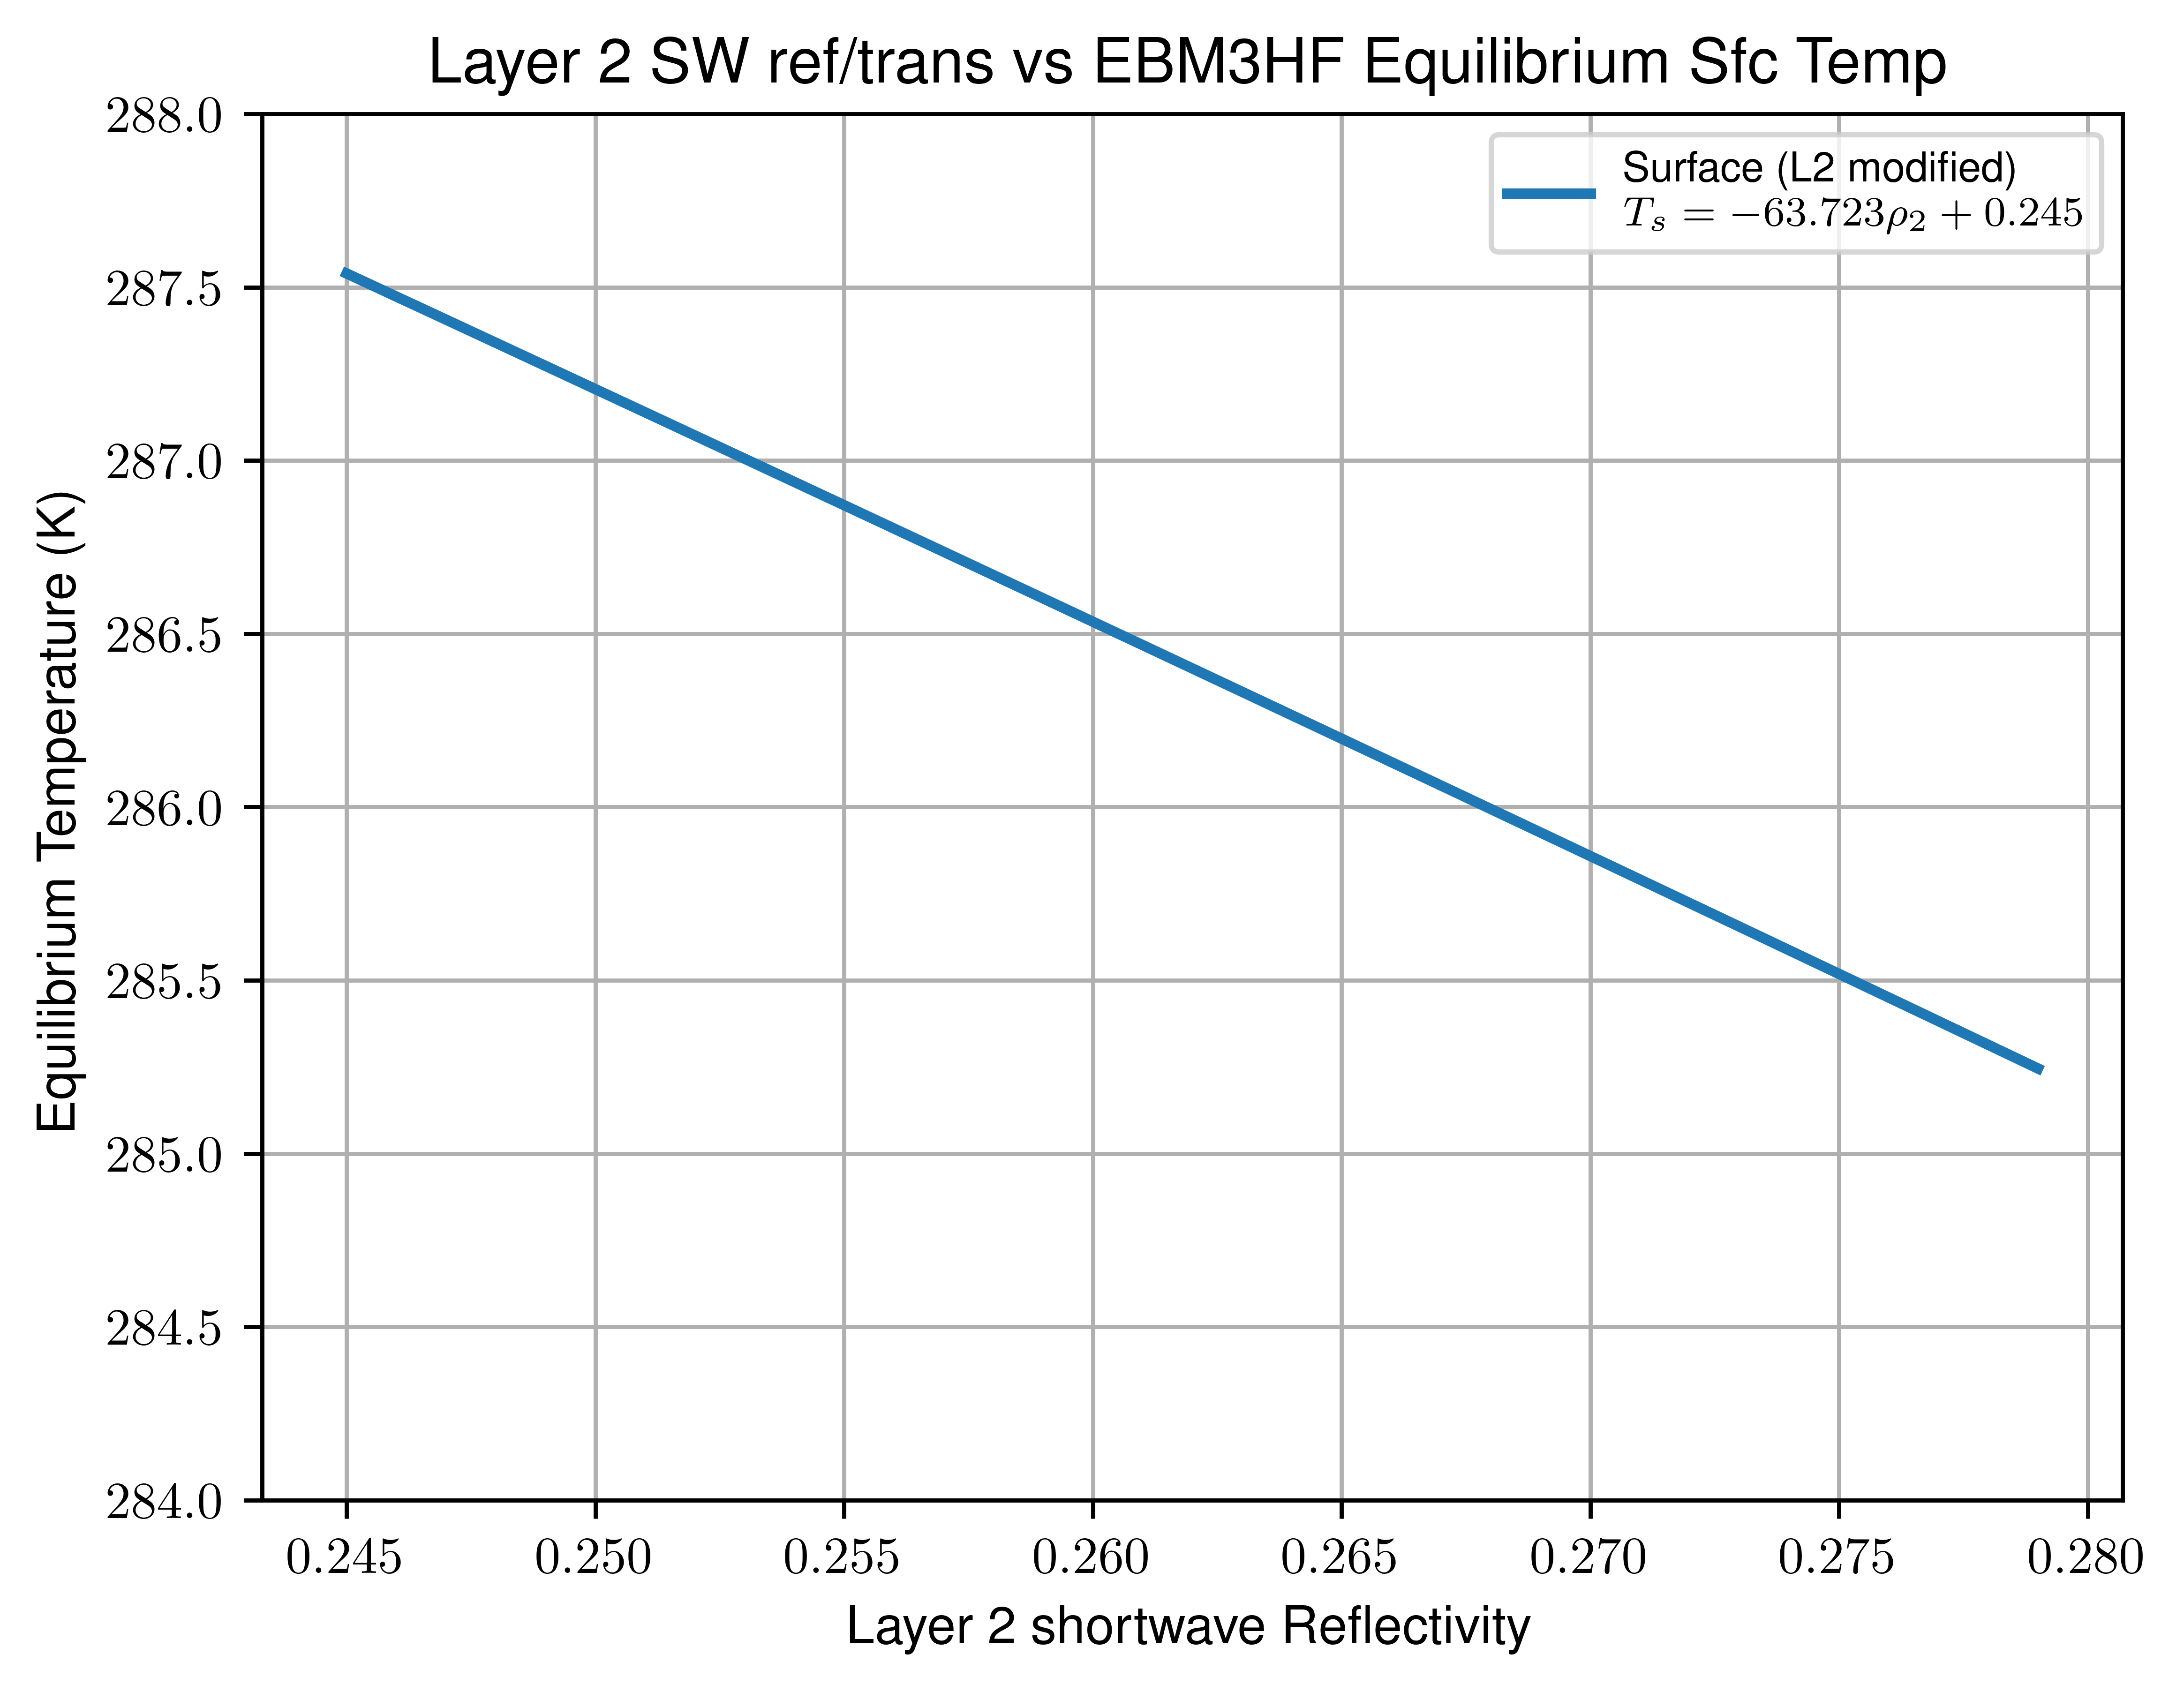
\includegraphics[width=.48\linewidth]{p1a.png}
    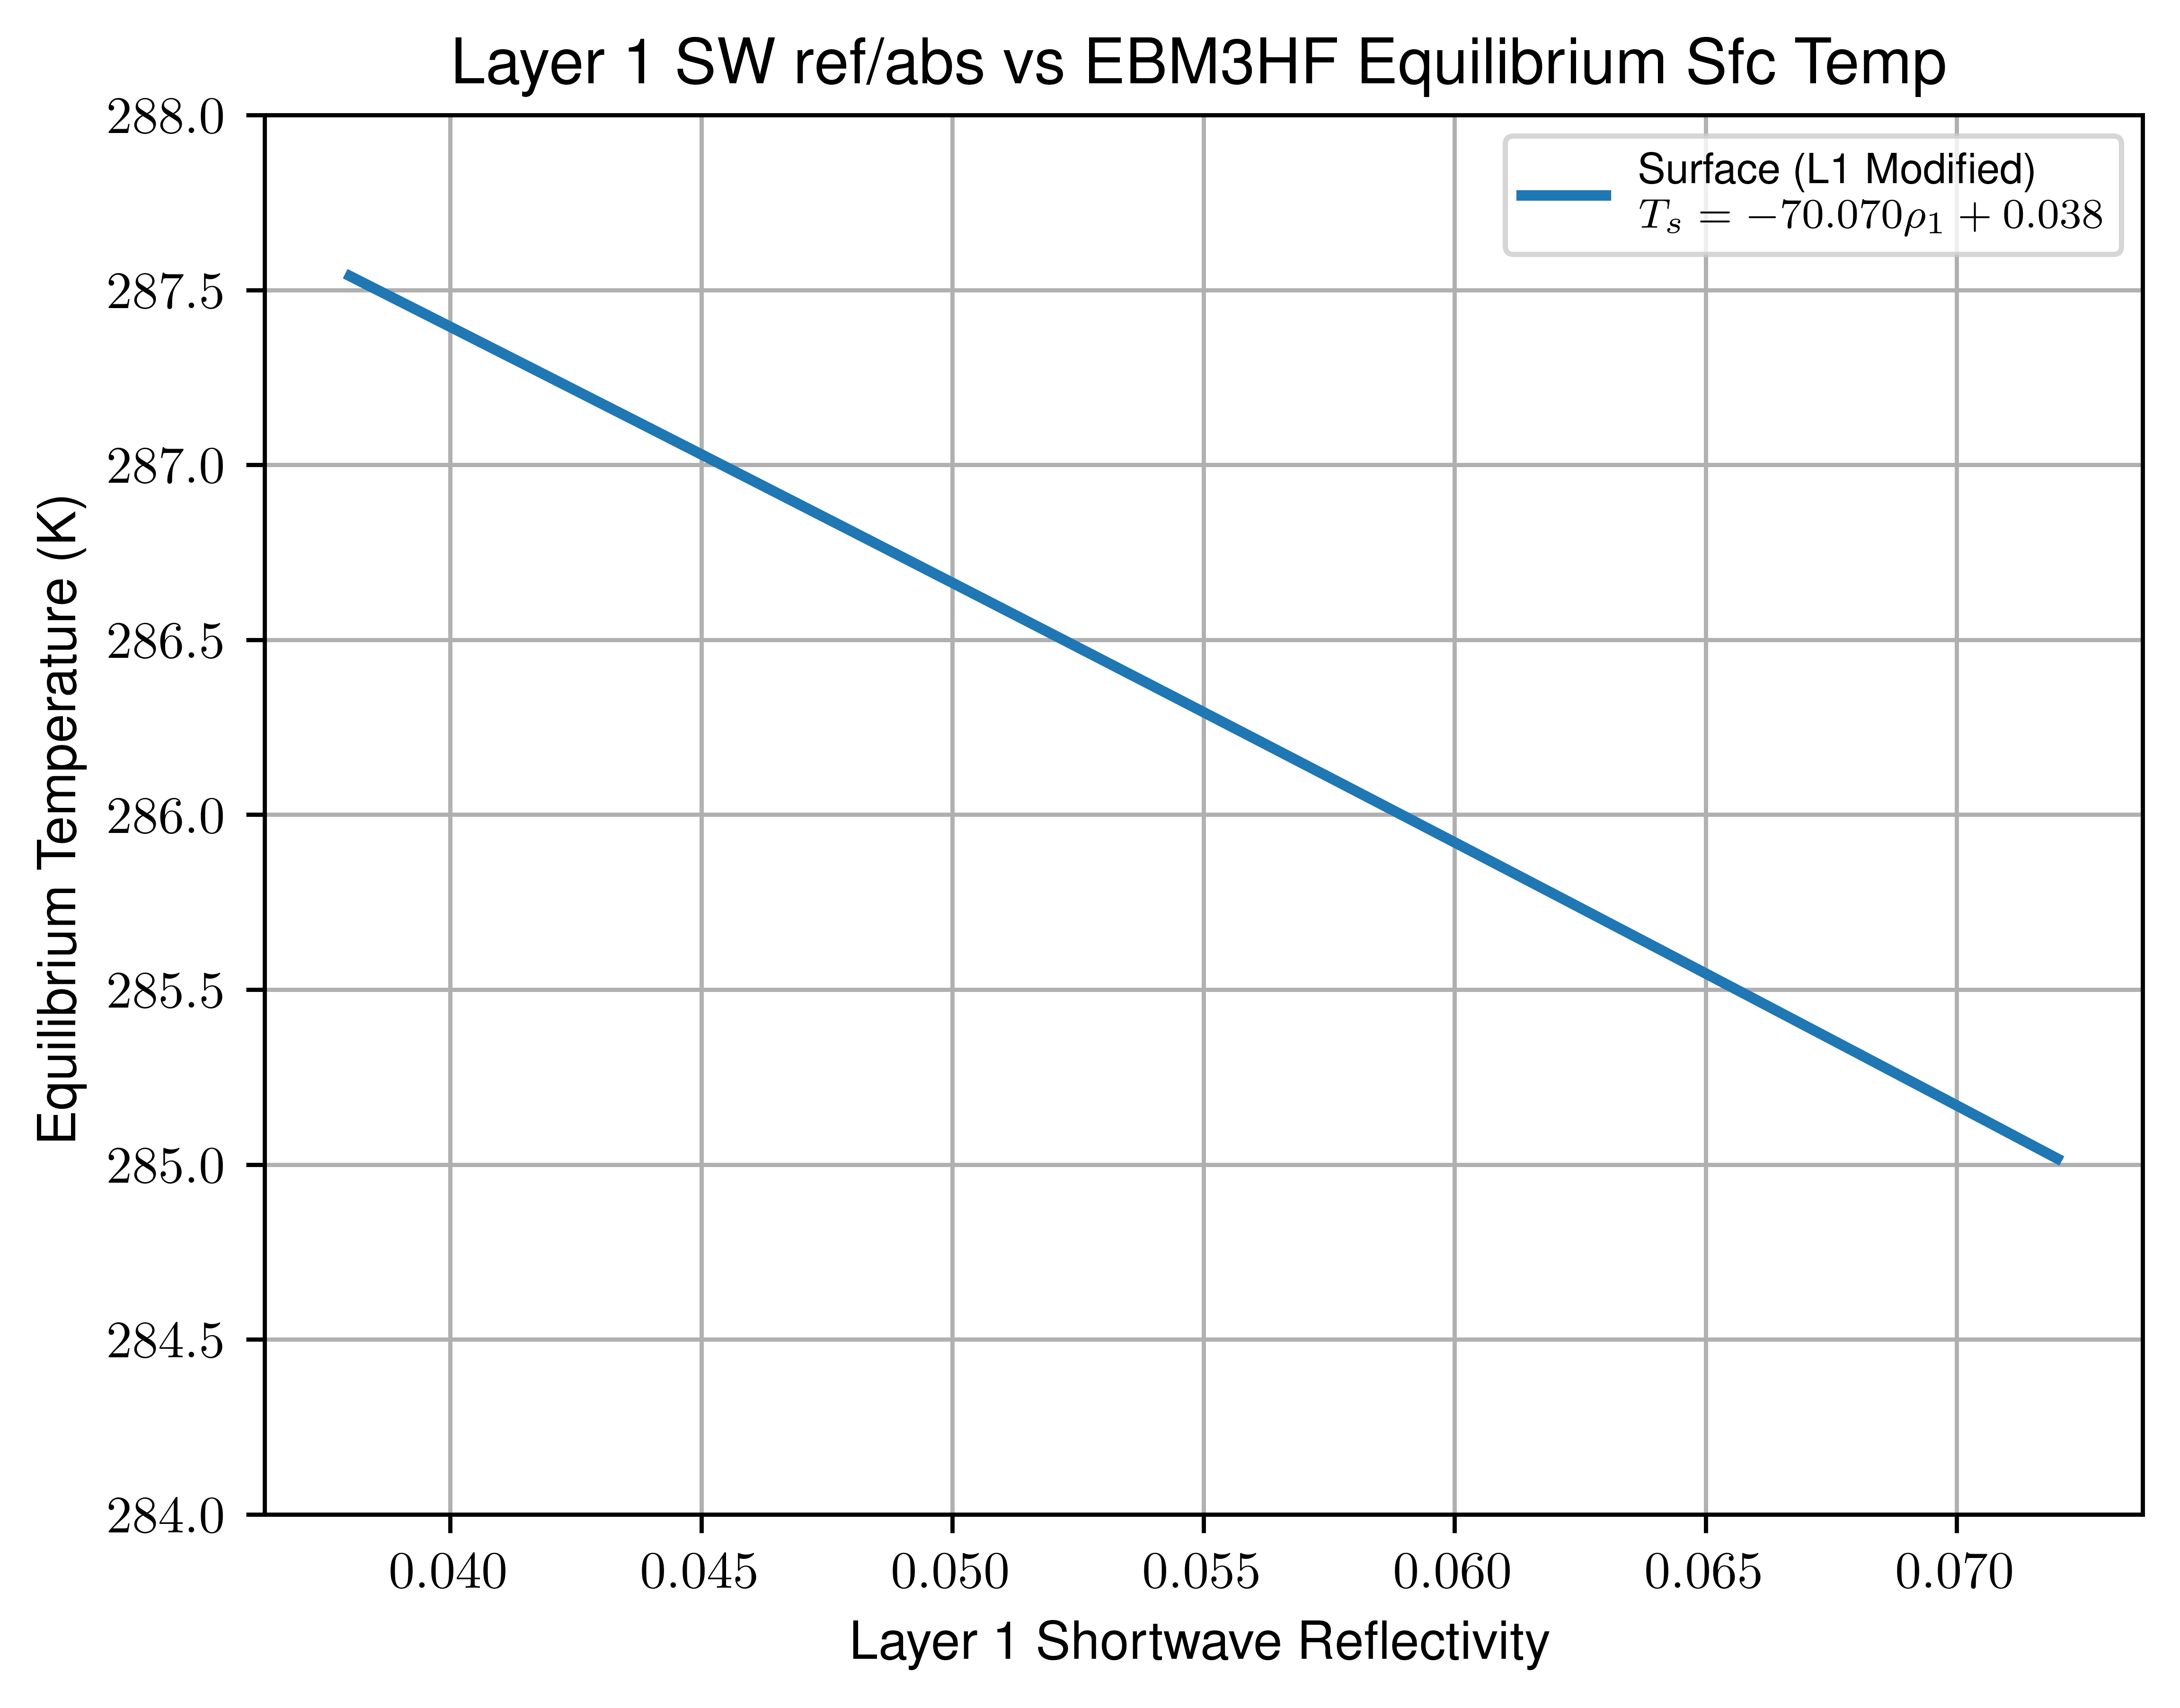
\includegraphics[width=.48\linewidth]{p1b.png}
    \caption{Change in surface temperature with respect to increases in layer 2 shortwave albedo (left), and layer 1 shortwave albedo (right), given the $EBM3_{HF}$ model with $Q=341\,\si{W.m^{-2}}$ and a heat exchange ratio of $0.287Q$.}
\end{figure}

The first image in Figure \ref{p1} models the surface temperature response to an increase in the ratio of tropospheric reflectivity in the shortwave spectrum as the absorptivity decreases. The overall effect is to decrease the surface's equilibrium temperature at an approximately linear rate of $-63.723\,\si{K}$ per reflectivity unit in range of the original reflectivity of $0.245$.

Since water vapor is the foremost absorbing constituent gas in the troposphere, one manifestation of the reduction of shortwave absorptivity could be a decrease in precipitable water vapor in the atmospheric column. Furthermore, an increase in the load of non-absorbing aerosols in the troposphere has the consequence of increasing the top-of-atmosphere albedo over most surface types. Since a reduction in precipitation due to lower water vapor content is associated with an increase in the lofting of dust-like continental aerosols by wind, one physical change that is consistent with the modeled effect is the aridification of a region.

The second image in Figure \ref{p1} shows the equilibrium surface temperature's response to increasing stratospheric albedo as stratospheric transmissivity decreases. The net effect is to decrease surface temperature at the slightly higher rate of $-70.07\,\si{K}$ per reflectivity unit, given an overall linear approximation in the range $\alpha_1 \in [0.038, 0.058]$.

Thinking outside of the stratosphere, one physical mechanism that could have a similar effect is a substantial increase in small metallic debris in or near the exosphere given a ``Kessler syndrome''-like event. In this eventuality, the collision of low earth orbit satellites hypothetically causes a cascading chain reaction by which exponentially more satellites are destroyed as a layer of fast-moving remnants gradually blankets common orbital zones. Until they eventually de-orbit due to minute friction, the often highly reflective debris would reduce the transmission of solar irradiance downward into the earth system, enhancing the reflectance of the corresponding layers similar to the above-modeled phenomenon.

\section{Offsetting Tropospheric Warming: Stratosphere}

\begin{figure}[h!]\label{p2}
    \centering
    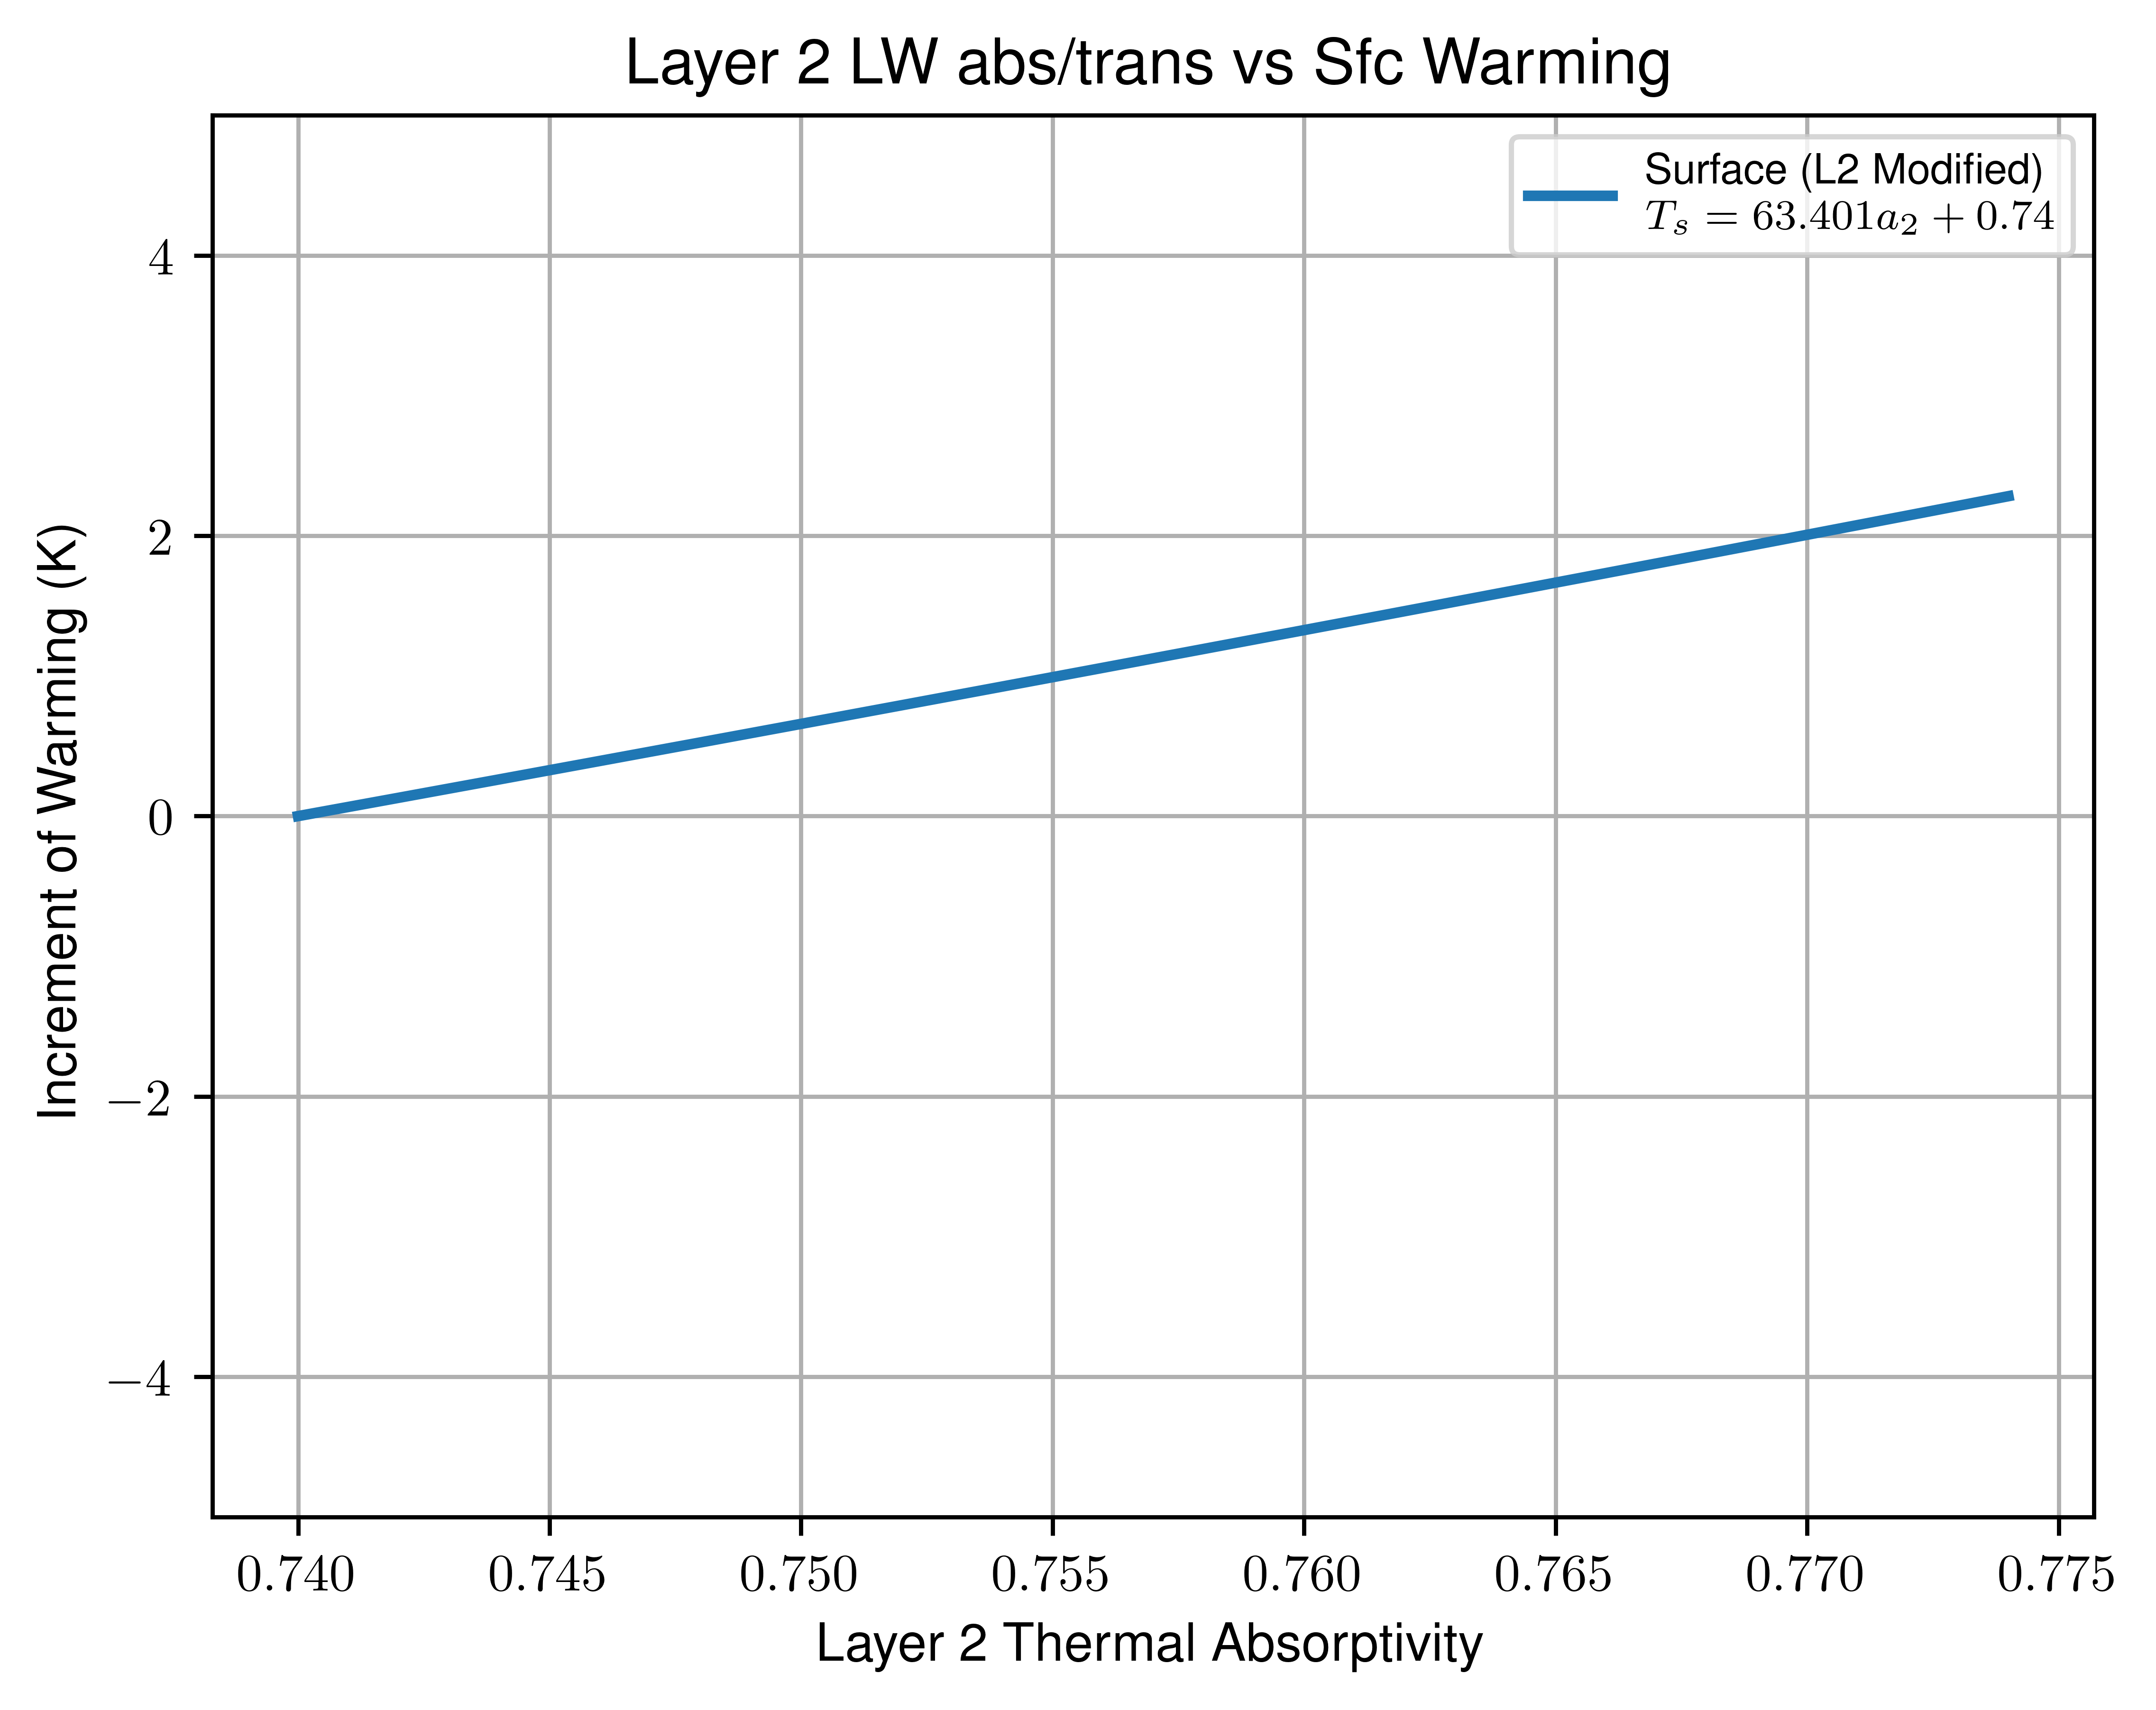
\includegraphics[width=.48\linewidth]{p2a.png}
    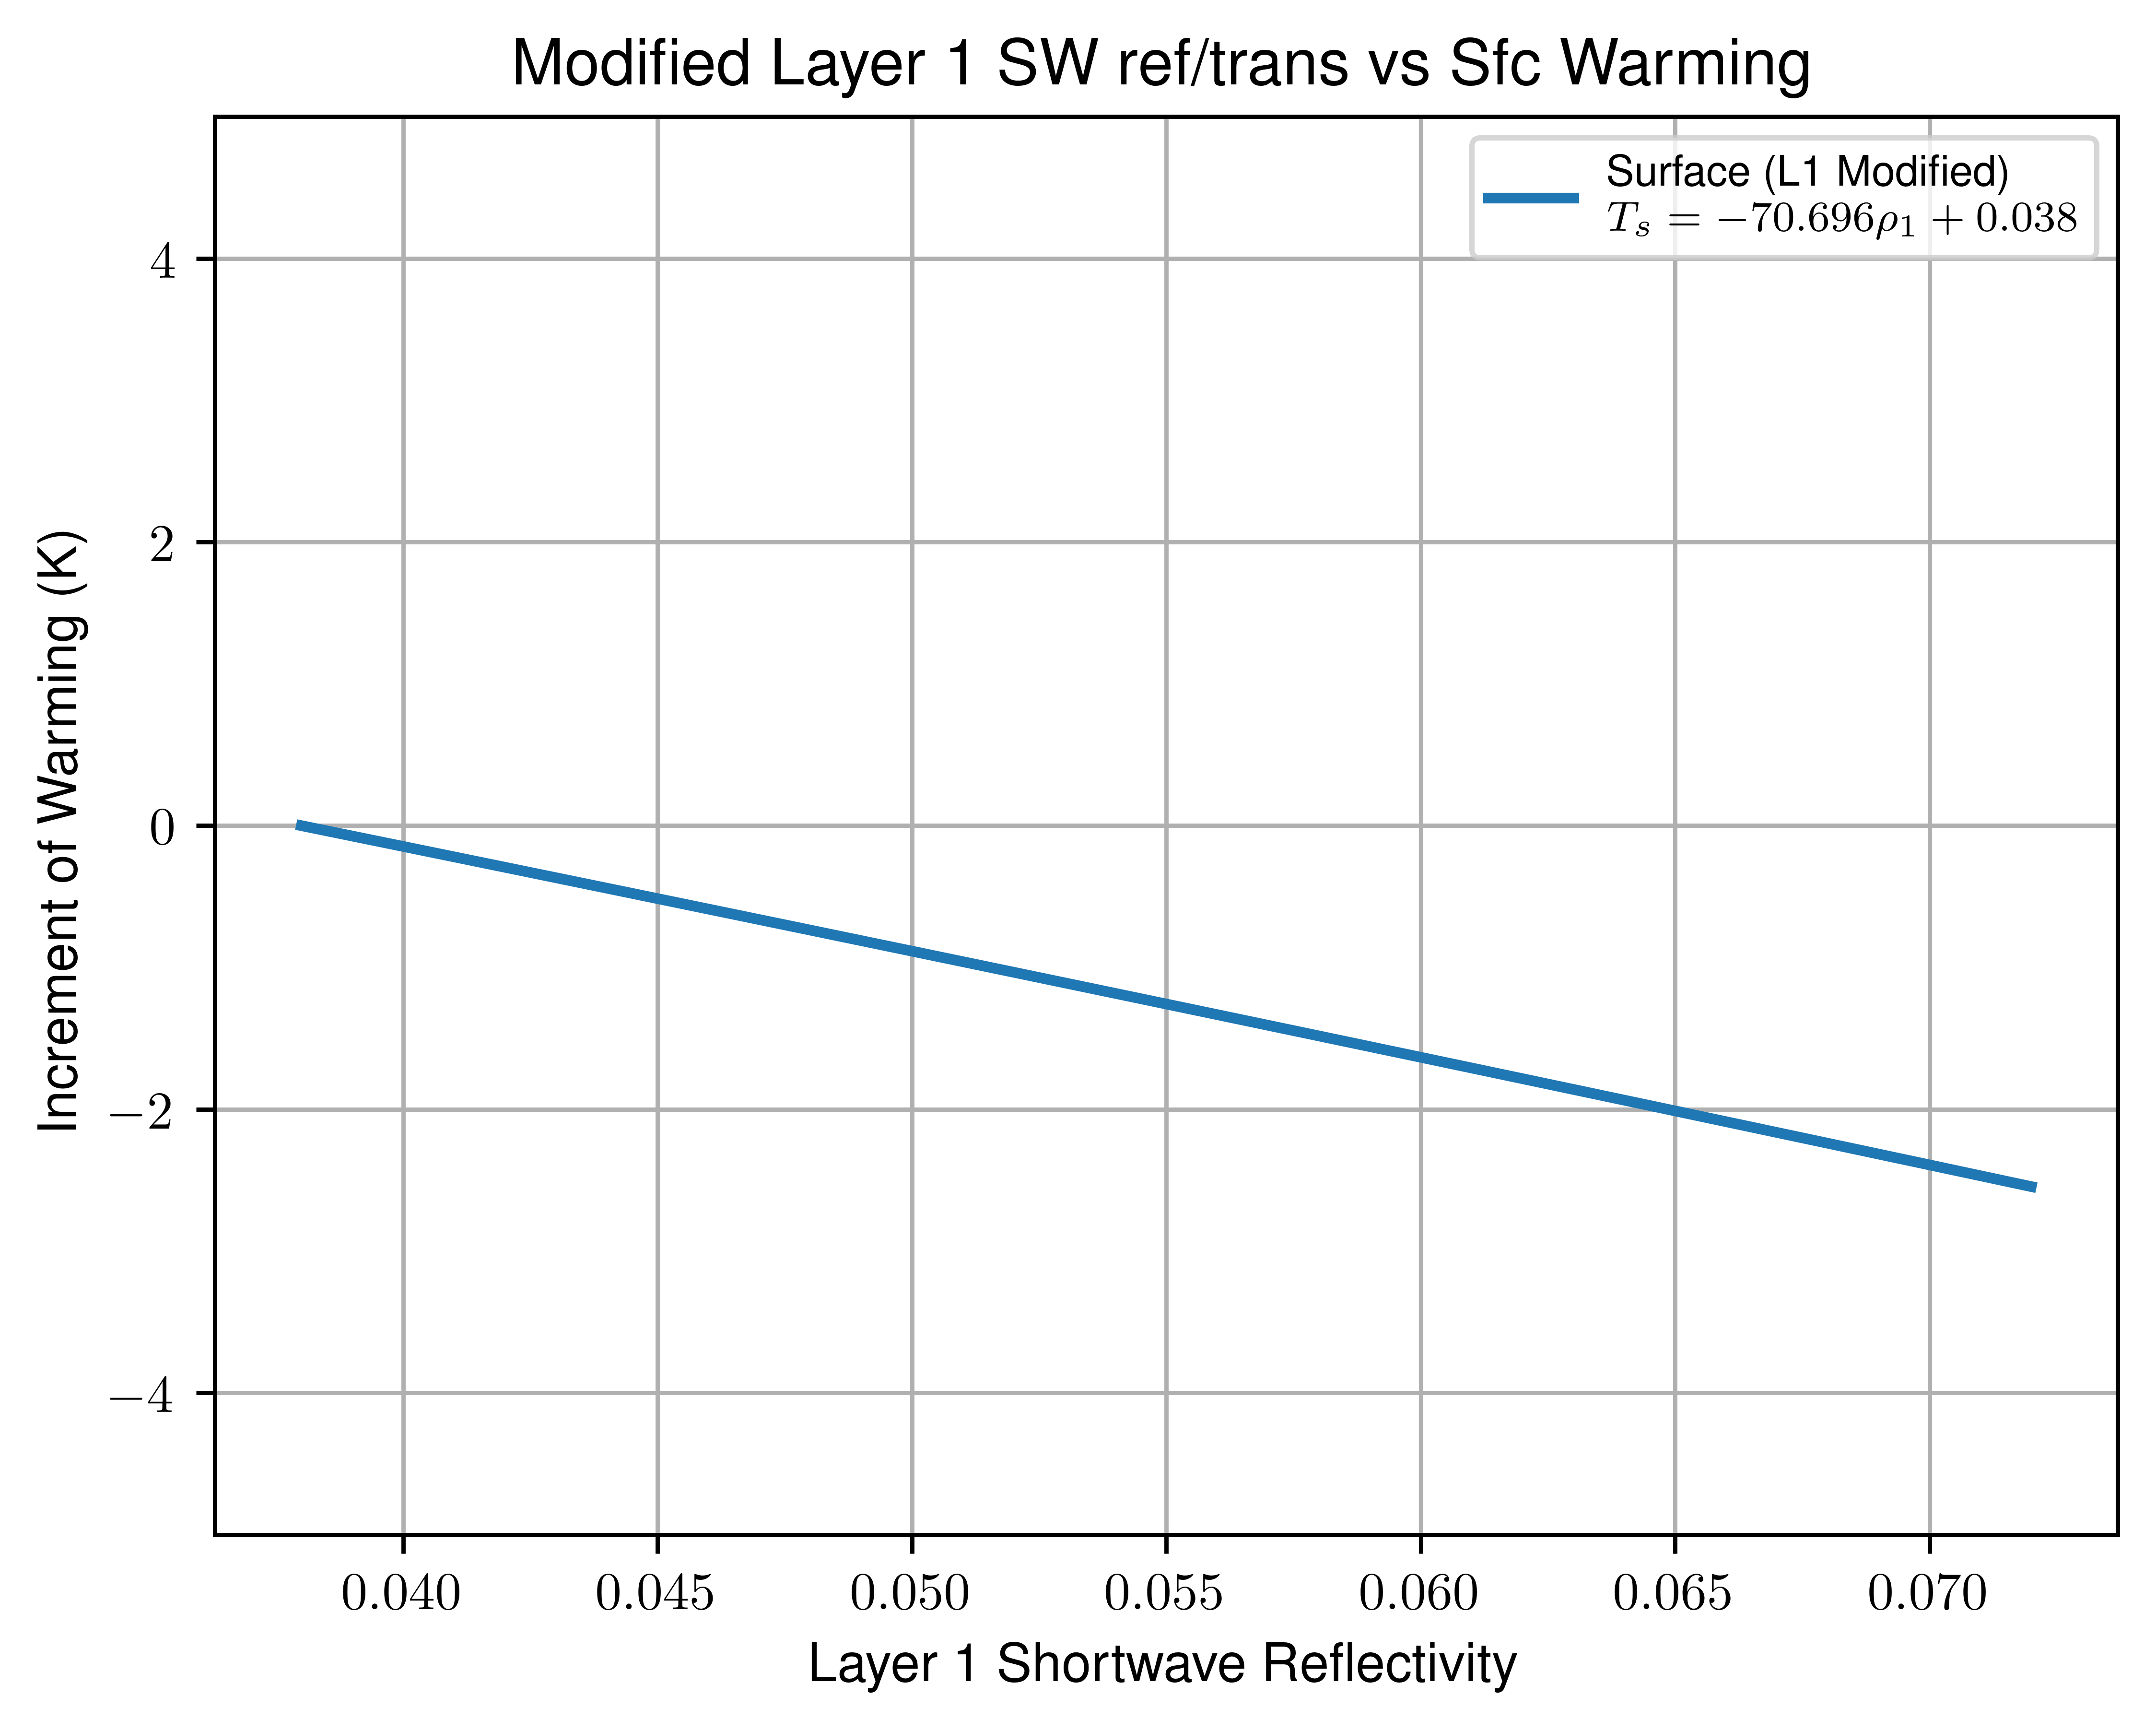
\includegraphics[width=.48\linewidth]{p2b.png}
    \caption{Increment of change in equilibrium surface temperature with enhanced layer 2 longwave absorptivity given baseline $EBM3_{HF}$ model (left). Also, subsequent increment of change in surface warming given an increase in layer 1 shortwave reflectivity (right).}
\end{figure}

Figure \ref{p2} first displays the total change in surface temperature after tropospheric absorptivity is increased to simulate the greenhouse effect. According to my $EBM3_{HF}$ implementation, a $+2\,\si{K}$ change in surface temperature is forced by an increase in longwave absorptivity coefficient of about $0.031$ as longwave transmissivity is reduced. Ultimately, the modified layer 2 infrared absorptivity is $.771$  and the transmissivity is $.014$.

The second image in Figure \ref{p2} starts with the above model with modified tropospheric absorptivity, and increases the stratosphere's solar reflectivity while decreasing its solar transmissivity. With a linear approximation, the change effects the surface temperature at a rate of about $-70.7\,\si{K}$ per reflectivity unit, so an increase in reflectivity of $0.028$ from $.038$ to $.066$ is needed to fully offset the $2\,\si{K}$ of warming.

\clearpage

\begin{figure}[h!]\label{p3p4}
    \centering
    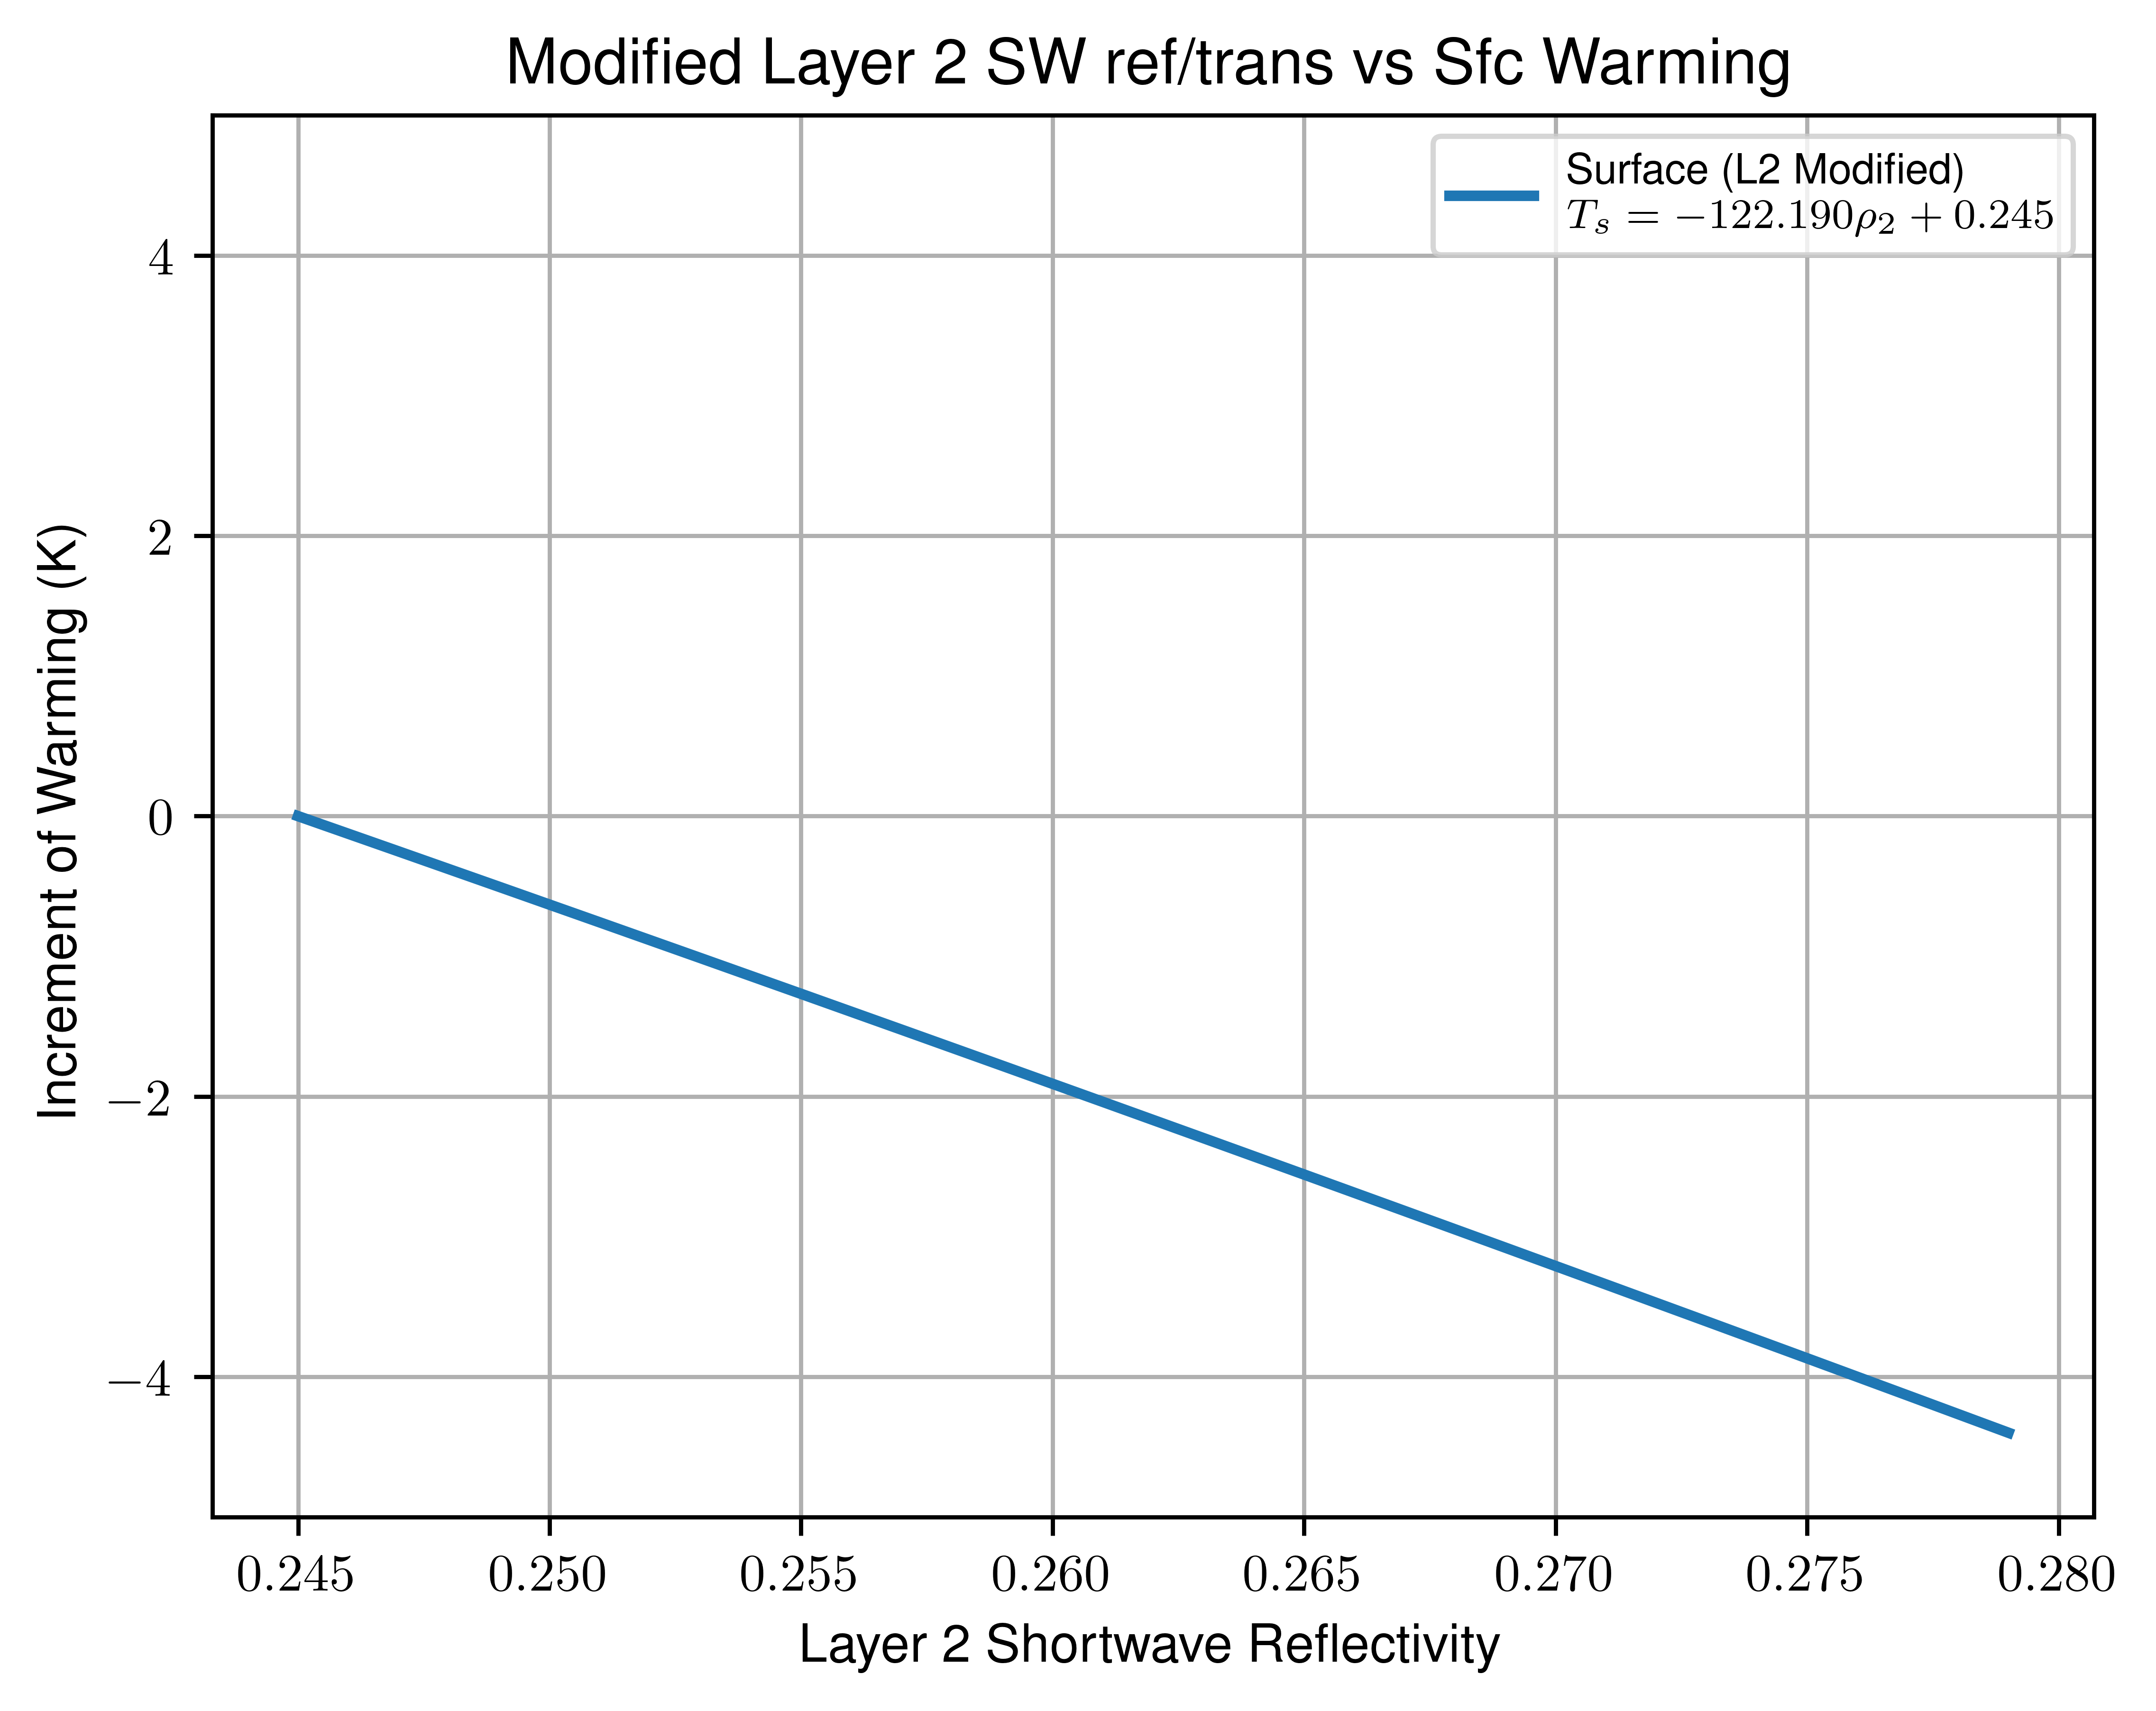
\includegraphics[width=.48\linewidth]{p3.png}
    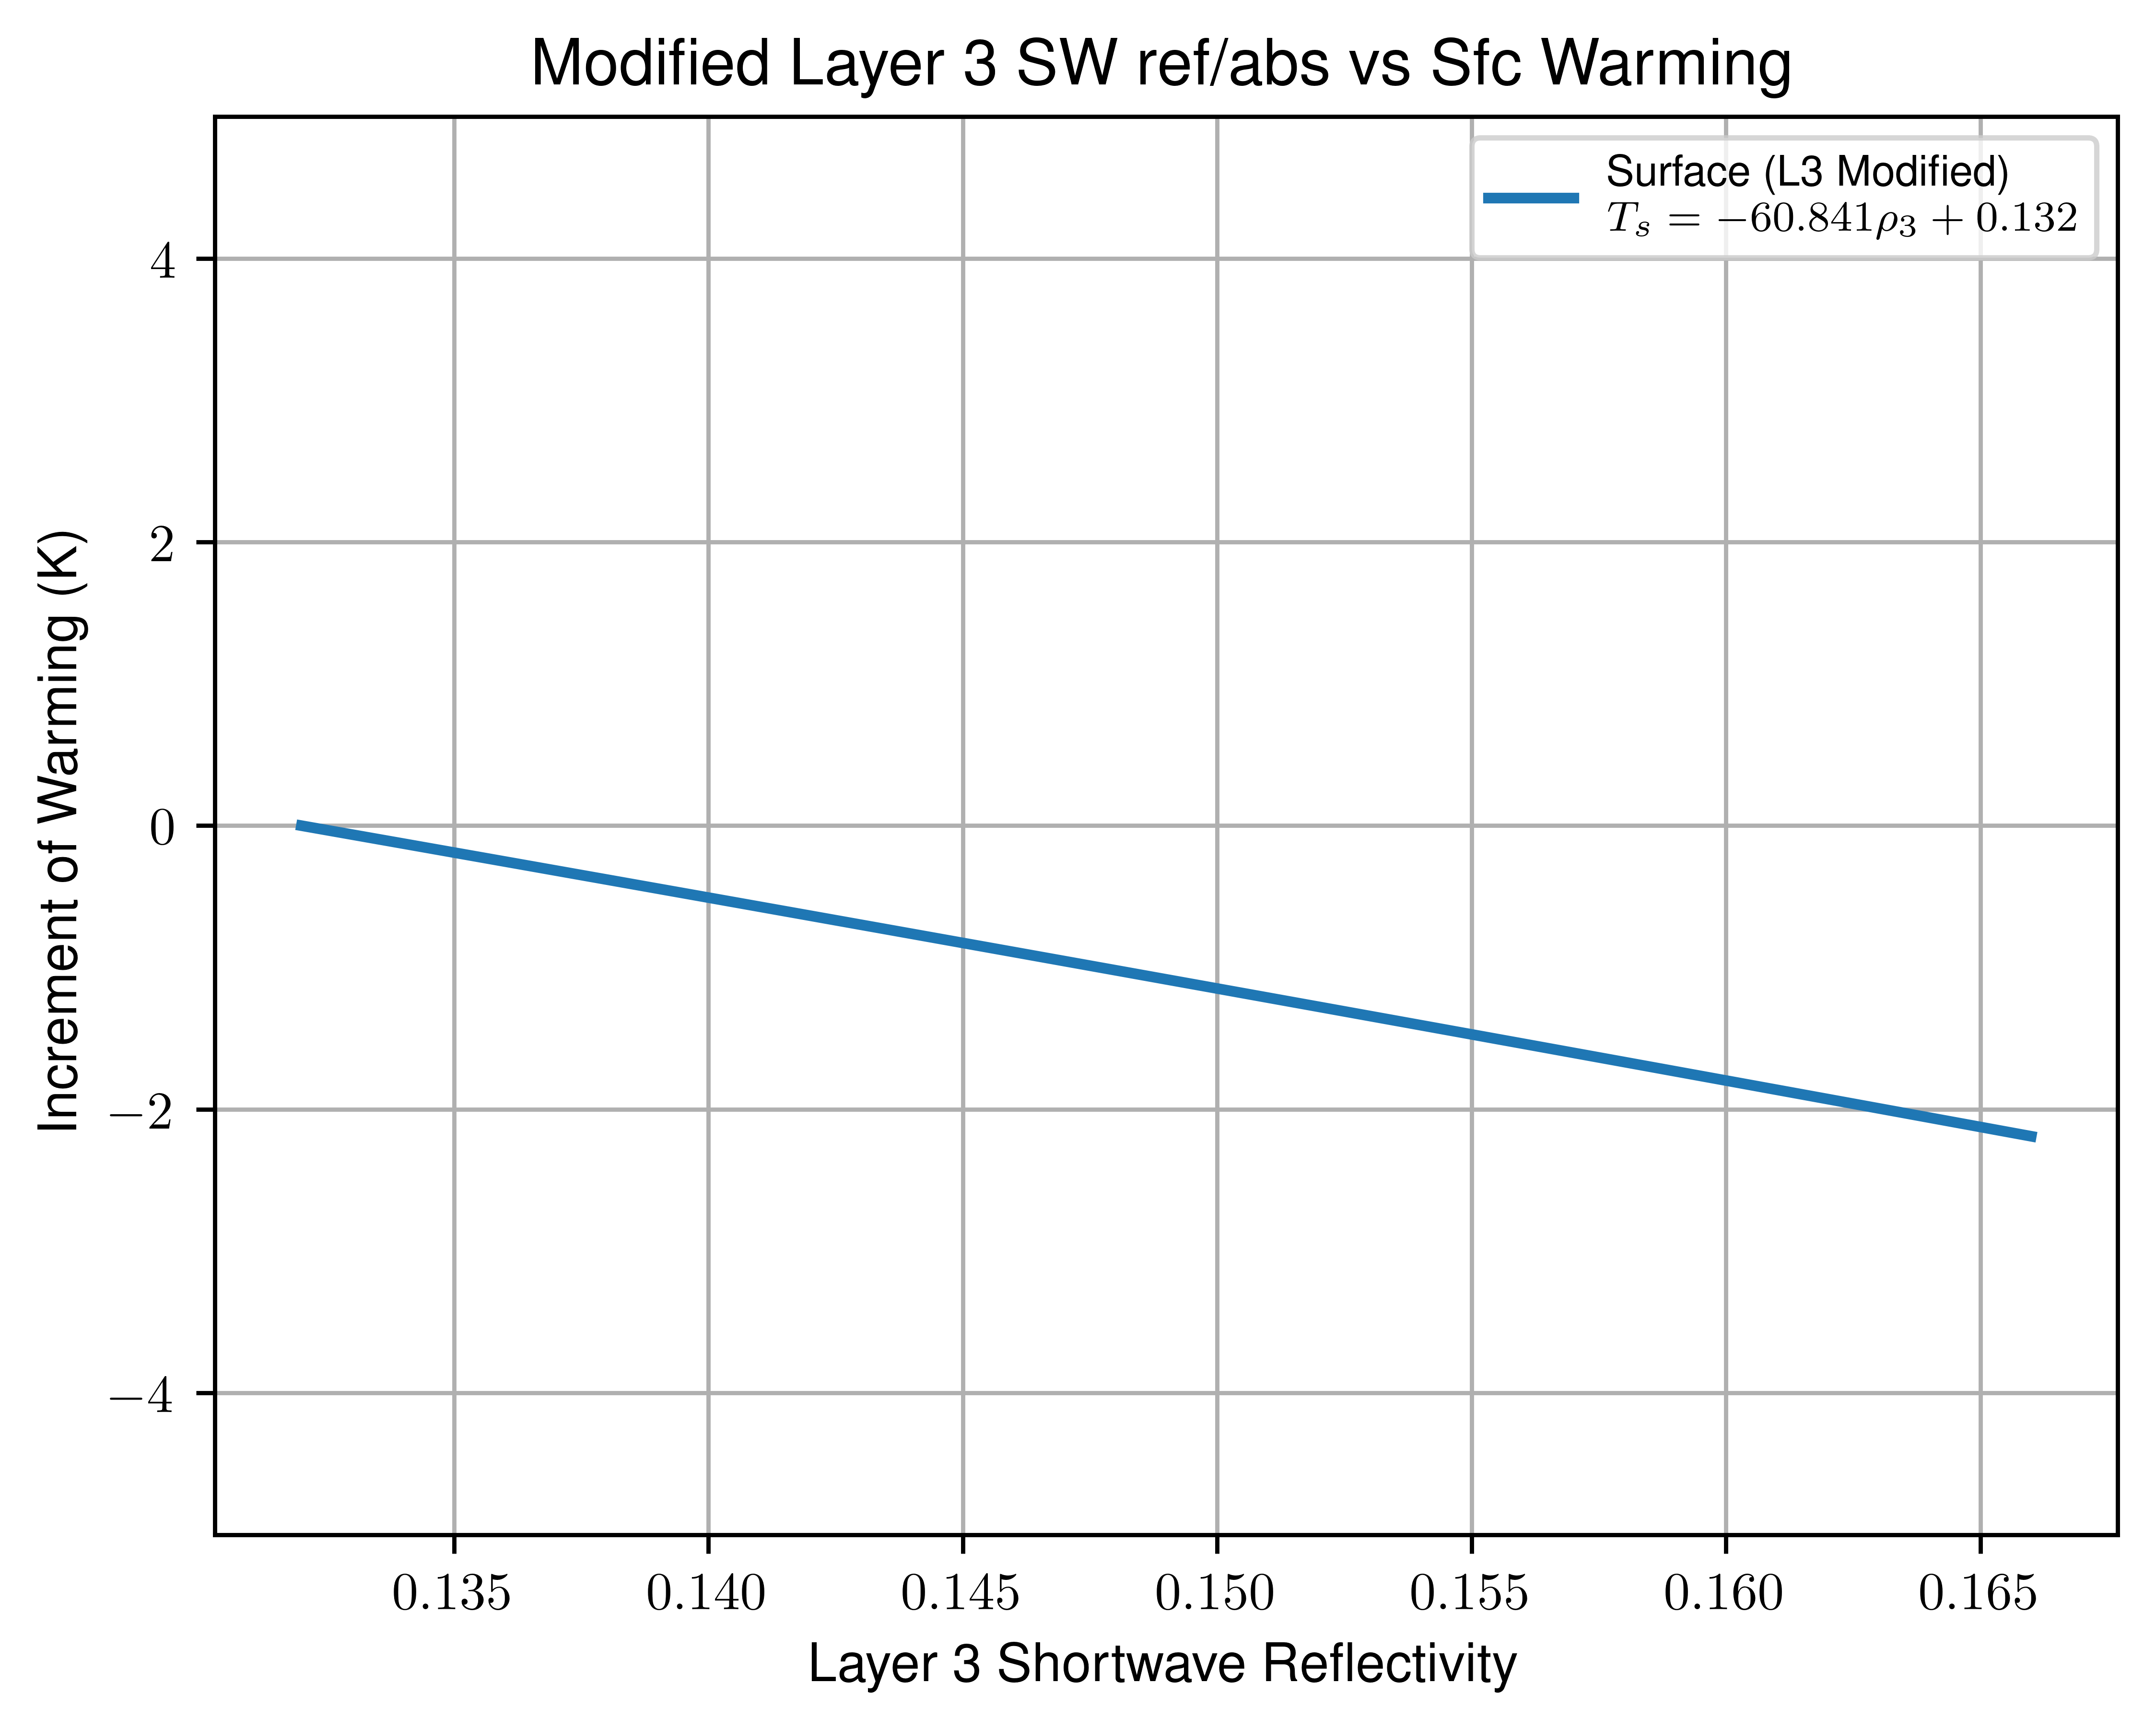
\includegraphics[width=.48\linewidth]{p4.png}
    \caption{Increments of change in equilibrium surface temperature with respect to $EBM3_{HF}$ model with modified tropospheric infrared absorption. Includes response to increase in layer 2 shortwave reflectivity (left) and layer 1 shortwave reflectivity (right).}
\end{figure}

\section{Offsetting Tropospheric Warming: Troposphere}

An increase in tropospheric cloud forcing and subsequent decrease in transmissivity is modeled in the left image of Figure \ref{p3p4}, which demonstrates the amount of surface temperature cooling with respect to the modified $EBM3_{HF}$ model from problem 2. The overall linear rate of change from the initial reflectance $\rho_2=0.245$ is approximately $-122.19\,\si{K}$ per tropospheric reflectance unit. In total, the tropospheric albedo must increase by $0.016$ to $\rho_2 = 0.261$ in order to fully offset the $2\,\si{K}$ warming from the simulated greenhouse effect.

\section{Offsetting Tropospheric Warming: Surface}

The right image of Figure \ref{p3p4} characterizes the effect on surface temperature of an increase in surface shortwave reflectance as shortwave absorptivity decreases. The results show a more modest rate of cooling at about $-60.84\,\si{K}$ per unit albedo increase around the initial albedo of $\rho_3 = 0.132$. This indicates that the surface reflectance needs to increase by about $0.033$ to $\rho_3 = 0.165$.

Ultimately, the results suggest that the surface temperature derived from the $EBM3_{HF}$ radiative model is most sensitive to incremental changes in tropospheric (layer 2) albedo by almost a factor of 2.

\end{document}

\begin{figure}[h!]\label{q1q2}
    \centering
    \begin{tabular}{ r | c | c c c}
        Model & Metric & Layer 1 & Layer 2 & Surface \T\B\\
        %\hline
        %\multicolumn{4}{c}{EBM3} \\
        \hline
        \multirow{2}*{EBM3$_0$} &
        Absorption ($\si{W.m^{-2}}$) & 8.714 & 59.969 & 170.158 \T\\
        & Temperature ($\si{K}$) & 233.716 & 269.503 & 308.461 \B\\
        %\hline
        %\multicolumn{4}{c}{EBM3 with Heat Flux} \\
        \hline
        \multirow{2}*{EBM3$_{HF}$} &
        Absorption ($\si{W.m^{-2}}$) & 8.713 & 158.859 & 71.268 \T\\
        & Temperature ($\si{K}$) & 233.716 & 271.120 & 287.295 \B\\
        \hline
        %\multicolumn{4}{c}{Kiehl and Trenberth 2} \\
        %\hline
        \multirow{2}*{K$\&$H 2} &
        Absorption ($\si{W.m^{-2}}$) & 10.547 & 174.976 & 48.809 \T\\
        & Temperature ($\si{K}$) & 243.985 & 286.226 & 286.587 \B\\
    \end{tabular}
    \caption{Layerwise equilibrium temperature and absorption of shortwave solar and heat flux energy for each of the coefficient sets of the 3-layer energy-based model. The absorption results for EBM3$_{HF}$ and Kiehl$\&$Trenberth 2 (K$\&$H 2) include heat flux from the surface to layer 2 such that HF$:=.29Q$ for average solar irradiance $Q=341\,\si{W.m^{-2}}$.}
\end{figure}
